\begin{titlepage}

\begin{center}
\vspace*{\fill}

\Huge Reverse Engineering \RU{для начинающих}\EN{for Beginners}

\bigskip
\bigskip

\begin{figure}[H]
\centering
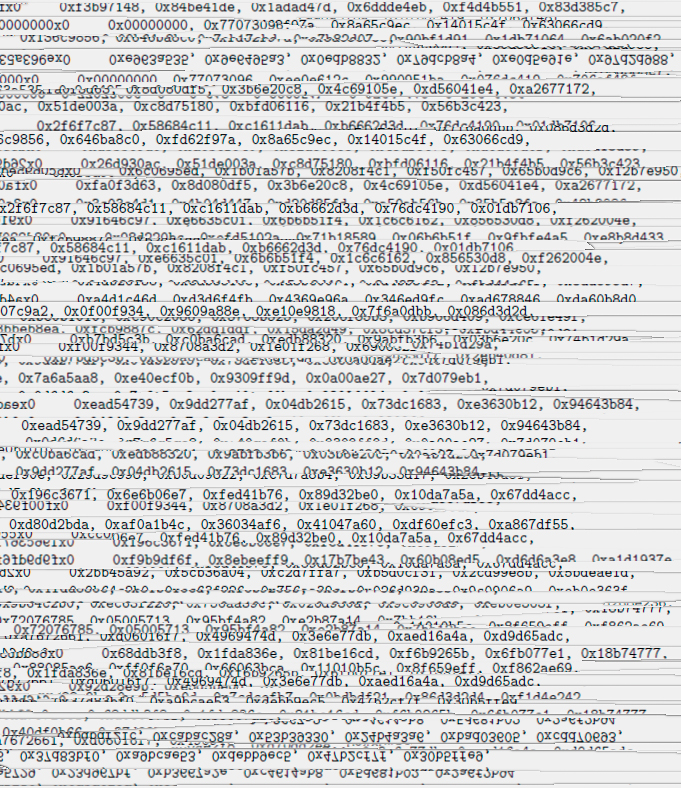
\includegraphics[scale=\FigScale]{cover.jpg}
\end{figure}

\bigskip

\hfill \huge \AUTHOR

\vspace*{\fill}
\end{center}

\end{titlepage}

\newpage

\begin{center}
\vspace*{\fill}
{\LARGE \TITLE}

\vspace*{\fill}

{\large \AUTHOR}

{\large \TT{<\EMAIL>}}
\vspace*{\fill}
\vfill

\ccbysa

\textcopyright 2013-2016, \AUTHOR. 

Questo lavoro è rilasciato sotto licenza Creative Commons Attribution-ShareAlike 4.0 International (CC BY-SA 4.0).
Per vedere la copia di questa licenza visita il sito \url{https://creativecommons.org/licenses/by-sa/4.0/}.

Teston ({\large \today}).

L'ultima versione (e l'edizione Russa) del testo sono accessibili al seguente sito: \href{http://go.yurichev.com/17009}{beginners.re}.
\ifdefined\ebook
Una copia in formato A4 è inoltre presente al sito sopra riportato.
\else
È inoltre disponibile una copia in formato A5 per gli e-book reader.
\fi

La copertina è stata creata da Andy Nechaevsky: \href{http://go.yurichev.com/17023}{facebook}.

\end{center}
